%%%%%%%%%%%%%%%%%%%%%%%%%%%%%%%%%%%%%%%%%
% Programming/Coding Assignment
% LaTeX Template
%
% This template has been downloaded from:
% http://www.latextemplates.com
%
% Original author:
% Ted Pavlic (http://www.tedpavlic.com)
%
% Note:
% The \lipsum[#] commands throughout this template generate dummy text
% to fill the template out. These commands should all be removed when 
% writing assignment content.
%
% This template uses a Perl script as an example snippet of code, most other
% languages are also usable. Configure them in the "CODE INCLUSION 
% CONFIGURATION" section.
%
%%%%%%%%%%%%%%%%%%%%%%%%%%%%%%%%%%%%%%%%%

%----------------------------------------------------------------------------------------
%	PACKAGES AND OTHER DOCUMENT CONFIGURATIONS
%----------------------------------------------------------------------------------------

\documentclass{article}

\usepackage{fancyhdr} % Required for custom headers
\usepackage{lastpage} % Required to determine the last page for the footer
\usepackage{extramarks} % Required for headers and footers
\usepackage[usenames,dvipsnames]{color} % Required for custom colors
\usepackage{graphicx} % Required to insert images
\usepackage{subcaption}
\usepackage{listings} % Required for insertion of code
\usepackage{courier} % Required for the courier font
\usepackage{lipsum} % Used for inserting dummy 'Lorem ipsum' text into the template
\usepackage{hyperref} % Used for linking to websites
\usepackage{amsmath, amsthm, amssymb} % Required for writing equations
\usepackage{pythonhighlight} % Required for including Python code
\usepackage{siunitx} % Required for scientific notation

% Margins
\topmargin=-0.45in
\evensidemargin=0in
\oddsidemargin=0in
\textwidth=6.5in
\textheight=9.0in
\headsep=0.25in

\linespread{1.1} % Line spacing

% Set up the header and footer
\pagestyle{fancy}
\lhead{\hmwkFirstAuthorName, \hmwkSecondAuthorName} % Top left header
\chead{\hmwkClass\ (\hmwkClassTime): \hmwkTitle} % Top center head
%\rhead{\firstxmark} % Top right header
\lfoot{\lastxmark} % Bottom left footer
\cfoot{} % Bottom center footer
\rfoot{Page\ \thepage\ of\ \protect\pageref{LastPage}} % Bottom right footer
\renewcommand\headrulewidth{0.4pt} % Size of the header rule
\renewcommand\footrulewidth{0.4pt} % Size of the footer rule

\setlength\parindent{0pt} % Removes all indentation from paragraphs

%----------------------------------------------------------------------------------------
%	CODE INCLUSION CONFIGURATION
%----------------------------------------------------------------------------------------

\definecolor{MyDarkGreen}{rgb}{0.0,0.4,0.0} % This is the color used for comments
\lstloadlanguages{Perl} % Load Perl syntax for listings, for a list of other languages supported see: ftp://ftp.tex.ac.uk/tex-archive/macros/latex/contrib/listings/listings.pdf
\lstset{language=Perl, % Use Perl in this example
        frame=single, % Single frame around code
        basicstyle=\small\ttfamily, % Use small true type font
        keywordstyle=[1]\color{Blue}\bf, % Perl functions bold and blue
        keywordstyle=[2]\color{Purple}, % Perl function arguments purple
        keywordstyle=[3]\color{Blue}\underbar, % Custom functions underlined and blue
        identifierstyle=, % Nothing special about identifiers                                         
        commentstyle=\usefont{T1}{pcr}{m}{sl}\color{MyDarkGreen}\small, % Comments small dark green courier font
        stringstyle=\color{Purple}, % Strings are purple
        showstringspaces=false, % Don't put marks in string spaces
        tabsize=5, % 5 spaces per tab
        %
        % Put standard Perl functions not included in the default language here
        morekeywords={rand},
        %
        % Put Perl function parameters here
        morekeywords=[2]{on, off, interp},
        %
        % Put user defined functions here
        morekeywords=[3]{test},
       	%
        morecomment=[l][\color{Blue}]{...}, % Line continuation (...) like blue comment
        numbers=left, % Line numbers on left
        firstnumber=1, % Line numbers start with line 1
        numberstyle=\tiny\color{Blue}, % Line numbers are blue and small
        stepnumber=5 % Line numbers go in steps of 5
}

% Creates a new command to include a perl script, the first parameter is the filename of the script (without .pl), the second parameter is the caption
\newcommand{\perlscript}[2]{
\begin{itemize}
\item[]\lstinputlisting[caption=#2,label=#1]{#1.pl}
\end{itemize}
}

%----------------------------------------------------------------------------------------
%	DOCUMENT STRUCTURE COMMANDS
%	Skip this unless you know what you're doing
%----------------------------------------------------------------------------------------

% Header and footer for when a page split occurs within a problem environment
\newcommand{\enterProblemHeader}[1]{
%\nobreak\extramarks{#1}{#1 continued on next page\ldots}\nobreak
%\nobreak\extramarks{#1 (continued)}{#1 continued on next page\ldots}\nobreak
}

% Header and footer for when a page split occurs between problem environments
\newcommand{\exitProblemHeader}[1]{
%\nobreak\extramarks{#1 (continued)}{#1 continued on next page\ldots}\nobreak
%\nobreak\extramarks{#1}{}\nobreak
}

\setcounter{secnumdepth}{0} % Removes default section numbers
\newcounter{homeworkProblemCounter} % Creates a counter to keep track of the number of problems
\setcounter{homeworkProblemCounter}{0}

\newcommand{\homeworkProblemName}{}
\newenvironment{homeworkProblem}[1][Part \arabic{homeworkProblemCounter}]{ % Makes a new environment called homeworkProblem which takes 1 argument (custom name) but the default is "Problem #"
\stepcounter{homeworkProblemCounter} % Increase counter for number of problems
\renewcommand{\homeworkProblemName}{#1} % Assign \homeworkProblemName the name of the problem
\section{\homeworkProblemName} % Make a section in the document with the custom problem count
\enterProblemHeader{\homeworkProblemName} % Header and footer within the environment
}{
\exitProblemHeader{\homeworkProblemName} % Header and footer after the environment
}

\newcommand{\problemAnswer}[1]{ % Defines the problem answer command with the content as the only argument
\noindent\framebox[\columnwidth][c]{\begin{minipage}{0.98\columnwidth}#1\end{minipage}} % Makes the box around the problem answer and puts the content inside
}

\newcommand{\homeworkSectionName}{}
\newenvironment{homeworkSection}[1]{ % New environment for sections within homework problems, takes 1 argument - the name of the section
\renewcommand{\homeworkSectionName}{#1} % Assign \homeworkSectionName to the name of the section from the environment argument
\subsection{\homeworkSectionName} % Make a subsection with the custom name of the subsection
\enterProblemHeader{\homeworkProblemName\ [\homeworkSectionName]} % Header and footer within the environment
}{
\enterProblemHeader{\homeworkProblemName} % Header and footer after the environment
}

%----------------------------------------------------------------------------------------
%	NAME AND CLASS SECTION
%----------------------------------------------------------------------------------------

\newcommand{\hmwkTitle}{Assignment\ \#2} % Assignment title
\newcommand{\hmwkDueDate}{Monday,\ February\ 18,\ 2018} % Due date
\newcommand{\hmwkClass}{CSC411} % Course/class
\newcommand{\hmwkClassTime}{L2501} % Class/lecture time
\newcommand{\hmwkFirstAuthorName}{Chawla Dhruv} % First name
\newcommand{\hmwkSecondAuthorName}{Lokman Sabrina} % First name

%----------------------------------------------------------------------------------------
%	TITLE PAGE
%----------------------------------------------------------------------------------------

\title{
\vspace{2in}
\textmd{\textbf{\hmwkClass:\ \hmwkTitle}}\\
\normalsize\vspace{0.1in}\small{Due\ on\ \hmwkDueDate}\\
\vspace{0.1in}
\vspace{3in}
}

\author{\textbf{\hmwkFirstAuthorName, \hmwkSecondAuthorName}}
%\date{} % Insert date here if you want it to appear below your name

%----------------------------------------------------------------------------------------

\begin{document}

\maketitle
\clearpage

%----------------------------------------------------------------------------------------
%   PART 1
%----------------------------------------------------------------------------------------

\begin{homeworkProblem}

\textit{Dataset Description}\\

The dataset consists of a set of images with each image representing a digit from $0$ to $9$.\\

Each image is 28x28 and has a black background with the digit handwritten in white.\\

Some of the images are straightforward to analyze and decipher while some are more tricky to ascertain what the handwriting is trying to represent (consider the 7th image from the left of the digit 5).\\

\begin{figure*}[h!]
    \centering
    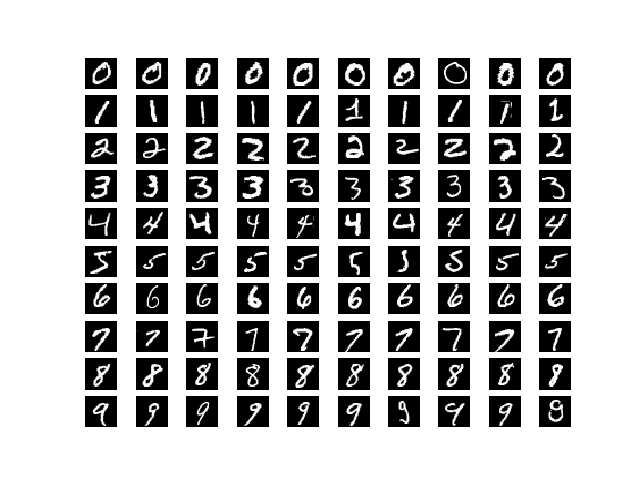
\includegraphics[scale=1]{part1.png}
    \caption{Images from the MNIST dataset}
    \label{fig:fig1}
\end{figure*}

\end{homeworkProblem}
\clearpage

%----------------------------------------------------------------------------------------
%   PART 2
%----------------------------------------------------------------------------------------

\begin{homeworkProblem}

\textit{Compute Simple Neural Network}\\

The function for computing simple neural network (no hidden layers) is in \texttt{mnist\_handout.py} and is reproduced here.\\

\begin{python}
def compute_simple_network(x, W, b):
    '''Compute a simple network (with no hidden layers)
    '''
    o = np.dot(W, x) + b
    return softmax(o)
\end{python}

An example of the function in action is seen below (and in \texttt{part2()} of \texttt{digits.py}).\\

\begin{verbatim}
>>> x = np.random.rand(784, 1)
>>> W = np.random.rand(10, 784)
>>> b = np.random.rand(10, 1)
>>> compute_simple_network(x, W, b).shape
(10, 1)
\end{verbatim}

\texttt{compute\_simple\_network(x, W, b)} returns the output layer of the neural network.\\

\end{homeworkProblem}
\clearpage

%----------------------------------------------------------------------------------------
%   PART 3
%----------------------------------------------------------------------------------------

\begin{homeworkProblem}

\textit{Cost Function: Sum of negative log-probabilities of all training cases}

\subsection{Part 3(a)}
Compute $\frac {\partial C} {\partial w_{ij}}$ (gradient of cost function with respect to a single weight)\\

For one training case, the cost function is (from slide 6 of One-Hot Encoding Lecture):

\begin{equation}
    C = - \sum_{j} y_{j} log p_{j}
\end{equation}

For $M$ training examples, the cost functions gets modified to:\\
\begin{equation}
    C = - \sum_{m=1}^M \sum_{j} y_{j} log p_{j}
\end{equation}

We also know that (from slide 7 of One-Hot Encoding Lecture), 

\begin{equation}
    p_{i} = \frac {e^{o_i}} {\sum_{j} e^{o_j}}
\end{equation}

The partial derivative will be the following:

\begin{equation}
    \frac {\partial p_i} {\partial o_j} = 
        \begin{cases}
            p_i (1 - p_i) &  i = j \\
            - p_i p_j &  i \ne j \
  \end{cases}
\end{equation}

Computing the cost function with respect to the output:
\begin{equation}
\frac {\partial C} {\partial o_i} = \sum_{j} \frac {\partial C} {\partial p_j}  \frac {\partial p_j} {\partial o_i}
\end{equation}

\begin{equation}
 = \frac {\partial C} {\partial p_i}  \frac {\partial p_i}{\partial o_i} - \sum_{j \ne i} \frac {\partial C} {\partial p_j}  \frac {\partial p_j}{\partial o_i}
\end{equation}

\begin{equation}
 = - y_i (1 - p_i) + \sum_{j \ne i} y_j p_j
\end{equation}

\begin{equation}
 = - y_i + p_i \sum_{j \ne i} y_j 
\end{equation}

\begin{equation}
 =  p_i - y_i 
\end{equation}

Computing the O with respect to weight
\begin{equation}
    o_{i} = \sum_{j} w_{ji} x_{j} + b
\end{equation}

\begin{equation}
    \frac {\partial o_i} {\partial w_{ij}} = \sum_j x_j
\end{equation}


Computing the cost function with respect to the weight
\begin{equation}
    \frac {\partial C} {\partial w_{ij}} =\sum_j \frac {\partial C} {\partial o_i} \frac {\partial o_i} {\partial w_{ij}} 
\end{equation}

we will get 
\begin{equation}
    \frac {\partial C} {\partial w_{ij}} = x_j (p_i - y_i)
\end{equation}

\clearpage

%__________________________________

\subsection{Part 3(b)}

\textit{Compute Gradient of Cost Function with respect to Weight}\\

The function for computing the gradient with respect to weight is in \texttt{mnist\_handout.py} and is reproduced here.\\

\begin{python}
def gradient_simple_network_w(x, W, b, y):
    p = compute_simple_network(x, W, b)

    gradient_mat = np.zeros((28*28, 10))

    for j in range(28*28):
        gradient_mat[j, :] = np.dot((p - y), x[j, :].T)

    return gradient_mat
\end{python}

\textit{Compute Gradient of Cost Function with respect to Bias}\\

The function for computing the gradient with respect to bias is in \texttt{mnist\_handout.py} and is reproduced here.\\

\begin{python}
def gradient_simple_network_b(x, W, b, y):
    p = compute_simple_network(x, W, b)

    return np.sum((p - y), axis=1).reshape((10, 1))
\end{python}

\end{homeworkProblem}
\clearpage

%----------------------------------------------------------------------------------------
%   PART 4
%----------------------------------------------------------------------------------------

\begin{homeworkProblem}

\textit{Train the neural network using Gradient Descent}\\

\begin{python}
def train_nn(f, df_W, df_b, x_train, y_train, x_test, y_test, init_W, init_b, alpha, max_iter = 2000):
    x = x_train
    y = y_train

    epoch, train_perf, test_perf = [], [], []

    EPS = 1e-10
    prev_W = init_W - 10 * EPS
    prev_b = init_b - 10 * EPS
    W = init_W.copy()
    b = init_b.copy()
    itr = 0

    while norm(W - prev_W) > EPS and norm(b - prev_b) > EPS and itr < max_iter:
        prev_W = W.copy()
        prev_b = b.copy()

        W -= alpha * df_W(x, W, b, y)
        b -= alpha * df_b(x, W, b, y)

        if itr % 500 == 0 or itr == max_iter - 1:
            epoch_i = itr
            train_perf_i = performance(x_train, W, b, y_train)
            test_perf_i = performance(x_test, W, b, y_test)

            epoch.append(epoch_i)
            train_perf.append(train_perf_i)
            test_perf.append(test_perf_i)

            print("Epoch: " + str(epoch_i))
            print("Training Performance:   " + str(train_perf_i) + "%")
            print("Testing Performance:    " + str(test_perf_i) + "%\n")

        itr += 1

    return W, b, epoch, train_perf, test_perf
\end{python}

\clearpage

Performance of the learning curves can be seen in figure $2$.

\begin{figure*}[h!]
    \centering
    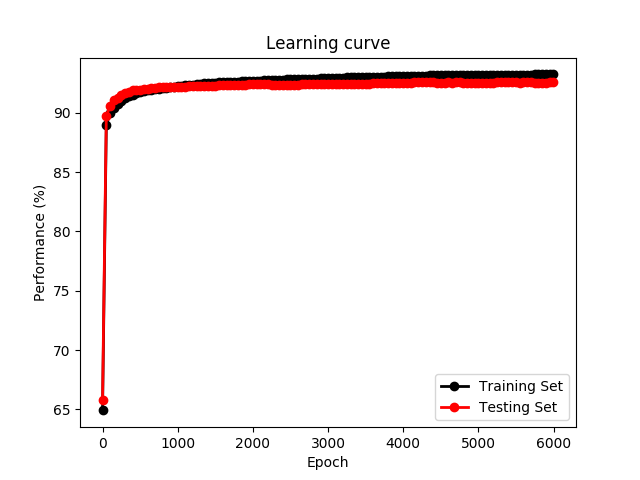
\includegraphics[scale=1]{part4_learning_curve.png}
    \caption{Learning curve for neural network using Gradient Descent}
    \label{fig:fig1}
\end{figure*}

\end{homeworkProblem}
\clearpage

%----------------------------------------------------------------------------------------
%   PART 5
%----------------------------------------------------------------------------------------

\begin{homeworkProblem}

\textit{Train the neural network using Gradient Descent with Momentum}\\

\begin{python}
def train_nn_M(f, df_W, df_b, x_train, y_train, x_test, y_test, init_W, init_b, alpha, gamma = 0.9, max_iter = 2000):
    x = x_train
    y = y_train

    epoch, train_perf, test_perf = [], [], []

    EPS = 1e-10
    prev_W = init_W - 10 * EPS
    prev_b = init_b - 10 * EPS
    W = init_W.copy()
    b = init_b.copy()
    itr = 0

    while norm(W - prev_W) > EPS and norm(b - prev_b) > EPS and itr < max_iter:
        prev_W = W.copy()
        prev_b = b.copy()

        W = (gamma * W) - alpha * df_W(x, W, b, y) 
        b -= alpha * df_b(x, W, b, y) 

        if itr % 200 == 0 or itr == max_iter - 1:
            epoch_i = itr
            train_perf_i = performance(x_train, W, b, y_train)
            test_perf_i = performance(x_test, W, b, y_test)

            epoch.append(epoch_i)
            train_perf.append(train_perf_i)
            test_perf.append(test_perf_i)

            print("Epoch: " + str(epoch_i))
            print("Training Performance:   " + str(train_perf_i) + "%")
            print("Testing Performance:    " + str(test_perf_i) + "%\n")

        itr += 1

    return W, b, epoch, train_perf, test_perf
\end{python}

\clearpage

Performance of the learning curves can be seen in figure $3$.

\begin{figure*}[h!]
    \centering
    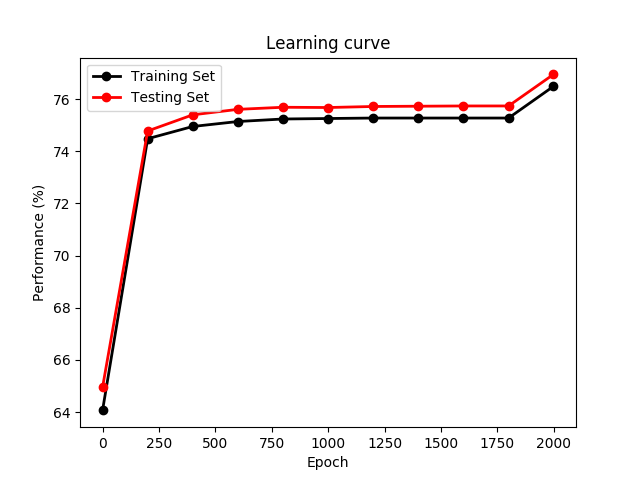
\includegraphics[scale=1]{part5_learning_curve.png}
    \caption{Learning curve for neural network using Gradient Descent with Momentum}
    \label{fig:fig1}
\end{figure*}

\end{homeworkProblem}
\clearpage

%----------------------------------------------------------------------------------------
%   PART 6
%----------------------------------------------------------------------------------------

\begin{homeworkProblem}

\end{homeworkProblem}
\clearpage

%----------------------------------------------------------------------------------------
%   PART 7
%----------------------------------------------------------------------------------------

\begin{homeworkProblem}

\end{homeworkProblem}
\clearpage

%----------------------------------------------------------------------------------------
%   PART 8
%----------------------------------------------------------------------------------------

\begin{homeworkProblem}

\end{homeworkProblem}
\clearpage

%----------------------------------------------------------------------------------------
%   PART 9
%----------------------------------------------------------------------------------------

\begin{homeworkProblem}

\end{homeworkProblem}
\clearpage

%----------------------------------------------------------------------------------------
%   PART 10
%----------------------------------------------------------------------------------------

\begin{homeworkProblem}

\end{homeworkProblem}
\clearpage

%----------------------------------------------------------------------------------------

\end{document}